%%
%% getstart.tex -- Flight Gear documentation: The FlightGear Manual
%% Chapter file
%%
%% Written by Michael Basler, started September 1998.
%%
%% Copyright (C) 2002 Michael Basler
%%
%%
%% This program is free software; you can redistribute it and/or
%% modify it under the terms of the GNU General Public License as
%% published by the Free Software Foundation; either version 2 of the
%% License, or (at your option) any later version.
%%
%% This program is distributed in the hope that it will be useful, but
%% WITHOUT ANY WARRANTY; without even the implied warranty of
%% MERCHANTABILITY or FITNESS FOR A PARTICULAR PURPOSE.  See the GNU
%% General Public License for more details.
%%
%% You should have received a copy of the GNU General Public License
%% along with this program; if not, write to the Free Software
%% Foundation, Inc., 675 Mass Ave, Cambridge, MA 02139, USA.
%%
%% $Id: free.tex,v 0.6 2002/09/09 michael
%% (Log is kept at end of this file)

%%%%%%%%%%%%%%%%%%%%%%%%%%%%%%%%%%%%%%%%%%%%%%%%%%%%%%%%%%%%%%%%%%%%%%%%%%%%%%%%%%%%%%%%%%%%%%%
\ifchinese
\chapter{{\\}想要自由的飞翔?玩 {\FlightGear{}} 吧!}
\fi
%\IfLanguageName{english}{
%\chapter{Want to have a free flight? Take {\FlightGear{}}!}
%}{}
\IfLanguageName{french}{
\chapter{Vous voulez voler librement ? Choisissez {\FlightGear{}} !}
}{}
\IfLanguageName{italian}{
\chapter{Vuoi avere un simulatore di volo libero? Usa {\FlightGear{}} !}
}{}
\label{free}
%%%%%%%%%%%%%%%%%%%%%%%%%%%%%%%%%%%%%%%%%%%%%%%%%%%%%%%%%%%%%%%%%%%%%%%%%%%%%%%%%%%%%%%%%%%%%%%

%%%%%%%%%%%%%%%%%%%%%%%%%%%%%%%%%%%%%%%%%%%%%%%%%%%%%%%%%%%%%%%%%%%%%%%%%%%%%%%%%%%%%%%%%%%%%%%
\ifchinese
\section{另一个飞行模拟器?}
\fi
%\IfLanguageName{english}{
%\section{Yet Another Flight Simulator?}
%}{}
\IfLanguageName{french}{
\section{Encore un autre simulateur de vol ?}
}{}
\IfLanguageName{italian}{
\section{Ancora un altro simulatore di volo?}
}{}
%%%%%%%%%%%%%%%%%%%%%%%%%%%%%%%%%%%%%%%%%%%%%%%%%%%%%%%%%%%%%%%%%%%%%%%%%%%%%%%%%%%%%%%%%%%%%%%
\ifchinese
\markboth{\thechapter.\hspace*{1mm} 想自由的飞翔?}{\thesection\hspace*{1mm}
另一个飞行模拟器?}
\fi
%\IfLanguageName{english}{
%\markboth{\thechapter.\hspace*{1mm} WANT TO HAVE A FREE FLIGHT?}{\thesection\hspace*{1mm}
%YET ANOTHER FLIGHT SIMULATOR?}
%}{}
\IfLanguageName{french}{
\markboth{\thechapter.\hspace*{1mm} VOUS VOULEZ VOLER LIBREMENT ?}{\thesection\hspace*{1mm}
ENCORE UN AUTRE SIMULATEUR DE VOL ?}
}{}

\ifchinese
你是否想过自己开飞机?但囿于金钱或者能力却望天兴叹?若你是个真实飞行员希望在地面提高自己的技术?或你是否希望挑战一些危险的动作,而不用担心生命安全?亦或你只是想体验一个没有暴力的严肃游戏?如果你符合以上任何问题,那么PC上的飞行模拟器对你就再适合不过了。

你也许已经用过 \Index{Microsoft}{\copyright} Flight Simulator(微软模拟飞行) 或者其他商业级 PC 飞行模拟器。这些模拟器大多 50 美元左右,买一个并不是什么大问题,然而为了运行这些飞行模拟器则需要电脑超强的硬件性能,而这些大概需要 1500 美元左右,即便现在硬件价格持续下跌。

既然已经有了这么多商业级的飞行模拟器,为什么我们还要花费数千小时编程和设计,开发一款自由的飞行模拟器呢?好吧,这里有很多原因,大体来说:
\fi
%\IfLanguageName{english}{
%Did you ever want to fly a plane yourself, but lacked the money or ability to do so? Are
%you a real pilot looking to improve your skills without having to take off? Do you want
%to try some dangerous maneuvers without risking your life? Or do you just want to have
%fun with a more serious game without any violence? If any of these questions apply
%to you, PC flight simulators are just for you.
%
%You may already have some experience using \Index{Microsoft}'s {\copyright} Flight Simulator
%or any other of the commercially available PC flight simulators. As the
%price tag of those is usually within the {\$}50 range, buying one of them should not be a
%serious problem given that running any serious PC flight simulator requires PC hardware
%within the {\$}1500 range, despite dropping prices.
%
%With so many commercially available flight simulators, why would we spend
%thousands of hours of programming and design work to build a free flight
%simulator?  Well, there are many reasons, but here are the major ones:
%}{}
%
\IfLanguageName{french}{
N'avez-vous jamais voulu piloter un avion par vous-m\^{e}me, mais manqu\'{e} d'argent ou de
comp\'{e}tences pour le faire ? Etes-vous un v\'{e}ritale pilote d\'{e}sirant progresser sans devoir
d\'{e}coller ? Voulez-vous tenter quelques man\oe{}uvres dangereuses sans risquer votre vie ?
Ou voulez-vous simplement vous amuser avec un jeu plus s\'{e}rieux sans aucune violence ?
Si l'une de ces questions s'applique \`{a} vous, alors les simulateurs de vol sur PC sont ce
qu'il vous faut.

Vous avez peut-\^{e}tre d\'{e}j\`{a} acquis de l'exp\'{e}rience aux commandes de \Index{Microsoft}
{\copyright} Flight Simulator ou d'un autre simulateur de vol sur PC disponible dans le commerce ?
Leurs prix se situant habituellement aux alentours de 70 euros, en acheter un ne devrait pas \^{e}tre
une grosse difficult\'{e}, en sachant que, malgr\'{e} la chute des prix, la configuration mat\'{e}rielle
exig\'{e}e pour faire fonctionner un simulateur de vol s\'{e}rieux sur PC revient \`{a} peu pr\`{e}s
\`{a} 1 000 euros.

Avec tant de simulateurs de vol disponibles sur le march\'{e}, pourquoi passer des milliers
d'heures de conception et de programmation pour construire un simulateur de vol libre et gratuit ?
Et bien, il y a de nombreuses raisons, mais en voici les principales :
}{}

\IfLanguageName{italian}{
Desideri pilotare un aereo da solo, ma non vuoi spendere denaro o non hai le capacit\`{a} per farlo?
Sei un vero pilota e stai cercando di migliorare le tue abilit\`{a} , senza dover decollare realmente?
Vuoi provare alcune manovre pericolose senza rischiare la vita?
O vuoi solo divertirti con un gioco pi\`{u} serio, senza alcun pericolo?
Se ad almeno una di queste domande la tua risposta \`{e} ''S\`{i}'', vuol dire che i simulatori di volo per
computer sono adatti per te.

Si pu\`{o} gi\`{a} avere una buona esperienza di volo con Microsoft Flight Simulator o con un qualsiasi
altro dei molti simulatori di volo per pc disponibili in commercio, ma nonostante il basso prezzo di uno
di questi (di solito circa 50\euro), si potrebbero avere problemi con l'hardware del computer in quanto sono
richiesti componenti di alta qualit\`{a}, che possono arrivare a costare anche 1500\euro.

Con cos\`{i} tanti simulatori di volo disponibili in rete, perch\'{e} avremmo dovuto spendere migliaia di
ore di programmazione e progettazione per costruire un simulatore di volo libero? Beh, ci sono molte
ragioni, ma qui sotto riportiamo quelle principali:
}{}

\begin{itemize}
\ifchinese
\fi
\item 所有商业飞行模拟器都有一个通病:由一群开发者根据自身的私有需要来定义什么对他们是重要的,并限制终端用户的接口。尝试联系一个商业开发者让他听你的声音,在这种情况下是一个巨大的挑战。然而 \FlightGear{} 是为所有人设计的,所有的一切都是开放的。
%\IfLanguageName{english}{
% \item All of the commercial simulators have a serious drawback: they are made
% by a small group of developers defining their properties according to what
% is important to them and providing limited interfaces to end users.  Anyone
% who has ever tried to contact a commercial developer would agree that getting
% your voice heard in that environment is a major challenge. In contrast,
% \FlightGear{} is designed by the people and for the people with everything
% out in the open.
%}{}
\IfLanguageName{french}{
 \item tous les simulateurs du commerce ont un inconv\'{e}nient majeur : ils sont
 con\c{c}us par un petit groupe de d\'{e}veloppeurs d\'{e}finissant leurs propri\'{e}t\'{e}s
 en fonction de ce qui leur est important et en fournissant des interfaces limit\'{e}es aux
 utilisateurs. Toute personne ayant d\'{e}j\`{a} essay\'{e} de contacter le d\'{e}veloppeur
 d'un logiciel du commerce sait que se faire entendre dans cet environnement est un r\'{e}el d\'{e}fi.
 \textit{A contrario}, \FlightGear{} est con\c{c}u par des utilisateurs et pour des utilisateurs,
 tout \'{e}tant fourni \textit{de base}.
}{}
\IfLanguageName{italian}{
  \item Tutti i simulatori commerciali hanno un grosso inconveniente: sono realizzati da un piccolo
  gruppo di sviluppatori che definiscono le loro caratteristiche in base a ci\`{o} che \`{e}
  importante per loro e forniscono interfacce limitate agli utenti finali. Chiunque abbia mai
  provato a contattare uno sviluppatore commerciale sarebbe d'accordo nel dire che far sentire
  la propria voce in questo ambiente rappresenta una grande sfida. Al contrario, FlightGear \`{e}
  stato progettato da un vasto gruppo di persone con tutti i codici liberamente disponibili e modificabili.
}{}

\ifchinese
\item 商业模拟器通常要在实用性和特性之间平衡。大多数商业开发者希望服务于更广泛的用户群,包括严肃的飞行员、初学者,甚至是休闲玩家。
而事实上,最终都会向期限和资金妥协。由于 \FlightGear{} 是自由且开放,也就没有了这些妥协。不会有发行商扼住我们的脖子,我们都是志愿者,大家一起制定自己的发行期限。我们也支持那些商业开发者没兴趣的领域,比如科研院所。
\fi
%\IfLanguageName{english}{
% \item Commercial simulators are usually a compromise of features and
% usability.  Most commercial developers want to be able to serve a broad
% segment of the population, including serious pilots, beginners, and even
% casual gamers.
% In reality the result is always a compromise due to deadlines and
% funding.  As \FlightGear{} is free and open, there is no need for such
% a compromise.  We have no publisher breathing down our necks, and
% we're all volunteers that make our own deadlines. We are also at
% liberty to support markets that no commercial developer would consider
% viable, like the scientific research community.
%}{}
\IfLanguageName{french}{
 \item les simulateurs commerciaux sont g\'{e}n\'{e}ralement un compromis
 entre fonctionnalit\'{e}s et facilit\'{e} d'utilisation. La majeure partie
 des \'{e}diteurs commerciaux veulent pouvoir toucher un large segment d'utilisateurs,
 comprenant de v\'{e}ritables pilotes, des d\'{e}butants et m\^{e}me des joueurs
 occasionnels.
 Au final, il y a donc toujours un compromis entre date de mise sur le march\'{e}
 et budget. Comme \FlightGear{} est libre et ouvert, il n'a aucun besoin de ce genre
 de compromis. Nous n'avons aucun \'{e}diteur sur le dos, nous sommes tous des
 volontaires qui d\'{e}finissons nous-m\^{e}mes nos propres dates de lancement. Nous
 sommes \'{e}galement libres de prendre en compte des march\'{e}s qu'aucun autre
 \'{e}diteur commercial ne consid\`{e}rerait rentable, comme la communaut\'{e} de la
 recherche scientifique.
}{}
\IfLanguageName{italian}{
  \item I simulatori commerciali solitamente sono un compromesso di funzionalit\`{a} e
  usabilit\`{a}, spesso a causa di scadenze e finanziamenti.
  La maggior parte degli sviluppatori commerciali vuole essere in grado di servire un ampio
  segmento della popolazione, compresi i piloti professionisti, i principianti, e anche i
  giocatori occasionali.
  Poich\'{e} FlightGear \`{e} libero e aperto, non vi \`{e} alcuna necessit\`{a} di un
  tale compromesso.
  Non abbiamo nessun editore che ci mette fretta, e siamo tutti volontari in grado di
  scegliere da soli le nostre scadenze.
}{}
\ifchinese
\item 因为它们的天然闭源,商业模拟器开发者将自己的天才想法和技能封闭的贡献给了他们的产品。在 \FlightGear{} 中,开发者的所有技术水平和想法对这个项目有巨大的潜在影响。贡献到一个如 \FlightGear{} 这样复杂的项目中是有非常丰厚报偿的,开发者将会因此获得巨大知名度,因为我们正打造一款伟大的模拟器。
\fi
%\IfLanguageName{english}{
% \item Due to their closed-source nature, commercial simulators keep developers
% with excellent ideas and skills from contributing to the products.  With
% \FlightGear{}, developers of all skill levels and ideas have the potential
% to make a huge impact on the project.  Contributing to a project as large
% and complex as \FlightGear{} is very rewarding and provides the developers
% with a great deal of pride in knowing that we are shaping the future of a
% great simulator.
%}{}
\IfLanguageName{french}{
 \item en raison de la fermeture de leur code source, les simulateurs du commerce
 doivent se passer de la contribution de d\'{e}veloppeurs imaginatifs et talentueux.
 Avec \FlightGear{}, des d\'{e}veloppeurs de tous niveaux et d\'{e}bordants d'id\'{e}es
 ont la possibilit\'{e} d'apporter des am\'{e}liorations \'{e}normes sur le projet.
 La contribution \`{a} un projet aussi grand et complexe que \FlightGear{} est une
 grande r\'{e}compense et offre aux d\'{e}veloppeurs la fiert\'{e} de participer au
 futur d'un grand simulateur.
}{}
\IfLanguageName{italian}{
  \item A causa della loro natura closed-source, nei simulatori commerciali solo gli sviluppatori
  pi\`{u} esperti possono contribuire a migliorare i prodotti.
  In FlightGear, invece, tutti gli sviluppatori, indipendentemente dal loro livello di
  abilit\`{a}, possono avere un enorme impatto sui progetti.
  Contribuire ad un progetto cos\`{i} grande e complesso come FlightGear \`{e} molto
  gratificante e offre ai programmatori un notevole orgoglio nel sapere che si sta
  plasmando il futuro di un ottimo simulatore.
}{}
\ifchinese
\item 除此之外,纯粹就是好玩!你也许拿我们和那些制作飞行套件或飞机图纸的真飞行员比较,当然我们可以去外面买一台预先造好的飞行器,然而自己做却有特殊的体验。
\fi
%\IfLanguageName{english}{
% \item Beyond everything else, it's just plain fun!  I suppose you could
% compare us to real pilots that build kit-planes or scratch-builts.  Sure,
% we can go out a buy a pre-built aircraft, but there's just something special
% about building one yourself.
%}{}
\IfLanguageName{french}{
 \item Enfin, et-au del\`{a} de ces consid\'{e}rations, c'est juste du pur plaisir ! Je suppose
 que vous pourriez nous comparer aux vrais pilotes qui assemblent des avions en kit ou qui construisent
 eux-m\^{e}mes leurs avions. Bien s\^{u}r, nous pourrions aller acheter un avion d\'{e}j\`{a} construit
 et par\'{e} \`{a} voler, mais il y a vraiment un sentiment si particulier quand on construit quelque
 chose de ses propres mains.
}{}
\IfLanguageName{italian}{
  \item Al di l\`{a} di tutto il resto, programmare questo simulatore \`{e} puro divertimento; certo,
  potevamo uscire di casa e comprare un gioco gi\`{a} fatto, ma abbiamo creduto che progettarne
  uno da soli avrebbe dato molta pi\`{u} soddisfazione.
}{}
\end{itemize}

\ifchinese
以上所列都是我们为什么要创建 \FlightGear{}。正是因为有了这些想法,我们想创建一个高质量的飞行模拟器。打造一个针对民用航空,\index{Flight simulator!civilian}跨平台的,\index{Flight simulator!multi-platform}开放的,\index{Flight simulator!open}用户支持的,\index{Flight simulator!user-supported}以及用户可扩展的,\index{Flight
  simulator!user-extensible}一个飞行模拟平台。
\fi
%\IfLanguageName{english}{
%  The points mentioned above form the basis of why we created \FlightGear{}.
%  With those motivations in mind, we have set out to create a high-quality
%  flight simulator that aims to be a civilian,\index{Flight simulator!civilian}
%  multi-platform,\index{Flight simulator!multi-platform} open,\index{Flight simulator!open}
%  user-supported,\index{Flight simulator!user-supported} and user-extensible\index{Flight
%  simulator!user-extensible} platform.  Let us take a closer look at each of these
%  characteristics:
%}{}
\IfLanguageName{french}{
  Les points mentionn\'{e}s ci-dessus forment la base des motivations pour lesquelles nous avons
  cr\'{e}\'{e} FlightGear. Avec ces motivations \`{a} l'esprit, nous nous sommes lanc\'{e}s dans
  la cr\'{e}ation d'un simulateur de vol de haute qualit\'{e} visant \`{a} \^{e}tre civil,\index{Flight simulator!civilian}
  multi-plateforme,\index{Flight simulator!multi-platform} ouvert,\index{Flight simulator!open}
  auto-maintenu,\index{Flight simulator!user-supported} et pouvant \^{e}tre \'{e}tendu par les utilisateurs
  eux-m\^{e}mes. Jetons un coup d'\oe{}il plus d\'{e}taill\'{e} \`{a} chacune de ces caract\'{e}ristiques :
}{}
\IfLanguageName{italian}{
  I punti menzionati in precedenza costituiscono la base del motivo per cui abbiamo creato FlightGear.

  Con queste motivazioni in mente, abbiamo deciso di creare un simulatore di volo di alta
  qualit\`{a} che mira ad essere civile, multipiattaforma, aperto, ideato per gli utenti,
  e open source. Diamo uno sguardo pi\`{u} da vicino a ciascuna di queste caratteristiche:
}{}

\begin{itemize}
\ifchinese
\item \textbf{民用航空:}\index{Flight simulator!civilian} 这个项目主要针对民用航空模拟。它适用于通用航空和民用客机。我们的长远打算是希望 \FlightGear{} 能成为 FAA 许可的飞行训练设备。某些用户会比较失望的是,\FlightGear{} 目前不是一个空战模拟器;不过相应的特性并非明确排除在外。我们只是没有开发者对空战模拟的系统性需求有严肃的兴趣。
\fi
%\IfLanguageName{english}{
% \item \textbf{Civilian:}\index{Flight simulator!civilian} The project is primarily aimed
% at civilian flight simulation.  It should be appropriate for simulating general aviation
% as well as civilian aircraft.  Our long-term goal is to have \FlightGear{} FAA-approved as
% a flight training device. To the disappointment of some users, it is currently not a
% combat simulator; however, these features are not explicitly excluded.  We just have
% not had a developer that was seriously interested in systems necessary for combat
% simulation.
%}{}
\IfLanguageName{french}{
 \item \textbf{Civil :}\index{Flight simulator!civilian} le projet vise essentiellement la
 simulation de vol civile. Il devrait permettre de simuler aussi bien l'aviation g\'{e}n\'{e}rale
 que civile. Notre but \`{a} long terme est de faire approuver \FlightGear{} par la FAA comme
 plateforme d'entra\^{i}nement au vol. Malheureusement pour les utilisateurs int\'{e}ress\'{e}s, ce
 n'est pas pour le moment un simulateur de combat; cependant, ces fonctionnalit\'{e}s ne sont pas
 explicitement exclues. C'est juste que nous n'avons pas eu de d\'{e}veloppeur s\'{e}rieusement
 int\'{e}ress\'{e} par les syst\`{e}mes n\'{e}cessaires \`{a} la simulation de combat.
}{}
\IfLanguageName{italian}{
  \item \textbf{Civile:} Il progetto si rivolge principalmente alle simulazioni di voli civili.
  Dovrebbe essere appropriato per simulare l'aviazione generale e la maggior parte degli aerei
  civili. Il nostro obiettivo a lungo termine \`{e} quello di ricevere la FAA (cio\`{e} la
  licenza che approva FlightGear come un dispositivo di addestramento al volo). Per la delusione
  di alcuni utenti, al momento non \`{e} un simulatore di combattimento, tuttavia, questa
  caratteristica non \`{e} esplicitamente esclusa. Noi semplicemente non siamo interessati a
  sistemi necessari per la simulazione di combattimenti.
}{}

\ifchinese
\item\textbf{跨平台:}\index{Flight simulator!multi-platform}开发者尝试让代码尽可能做到平台无关性。根据我们的观察,对飞行模拟感兴趣的人运行了各种计算机硬件和操作系统,本项目代码支持如下\Index{操作系统}:
 \begin{itemize}
  \item\Index{Linux} (任何发行版和平台),
  \item\Index{Windows NT/2000/XP/7} (Intel/AMD 平台),
  \item\Index{Windows 95/98/ME},
  \item\Index{BSD UNIX},
  \item\Index{Sun-OS},
  \item{Mac OS X}
  \end{itemize}
目前为止,还没有任何一个飞行模拟器——无论是商业的或者自由的——能够支持如此广泛的平台。
\fi
%\IfLanguageName{english}{
% \item\textbf{Multi-platform:}\index{Flight simulator!multi-platform} The
% developers are attempting to keep the code as platform-independent as poss%ible. This
% is based on their observation that people interested in flight simulations% run quite a
% variety of computer hardware and operating systems. The present code suppo%rts the
% following \Index{Operating Systems}:
%  \begin{itemize}
%  \item\Index{Linux} (any distribution and platform),
%  \item\Index{Windows NT/2000/XP/Seven} (Intel/AMD platform),
%  \item\Index{Windows 95/98/ME},
%  \item\Index{BSD UNIX},
%  \item\Index{Sun-OS},
%  \item{Mac OS X}
%  \end{itemize}
%At present, there is no other known flight simulator -- commercial or free
%-- supporting such a broad range of platforms.
%}{}
\IfLanguageName{french}{
 \item\textbf{Multi-platformes :}\index{Flight simulator!multi-platform} les
 d\'{e}veloppeurs essayent de maintenir le code aussi ind\'{e}pendant que
 possible de la plate-forme. Cette motivation est bas\'{e}e sur leur observation
 que les gens int\'{e}ress\'{e}s par la simulation de vol utilisent toute une vari\'{e}t\'{e} de
 mat\'{e}riel informatique et de syst\`{e}mes d'exploitation. Le code actuel prend en charge les
 \Index{Syst\`{e}mes d'exploitation} suivants :
  \begin{itemize}
  \item\Index{Linux} (toutes distributions et plate-formes),
  \item\Index{Windows NT/2000/XP/Seven} (plate-formes Intel/AMD),
  \item\Index{Windows 95/98/ME},
  \item\Index{BSD UNIX},
  \item\Index{Sun-OS},
  \item{Mac OS X}
  \end{itemize}
A notre connaissance, il n'existe pas aujourd'hui d'autre simulateur de vol, commercial ou libre,
prenant en charge une gamme aussi \'{e}tendue de plate-formes.
}{}
\IfLanguageName{italian}{
  \item\textbf{Multipiattaforma: }\index{Flight simulator!multi-platform} Gli sviluppatori
  stanno cercando di mantenere il codice indipendente dalla piattaforma il pi\`{u} possibile.
  Questo per permettere di usare il simulatore di volo su tutti i computer, indistintamente
  dal sistema operativo o dall'hardware usato. Il codice attuale supporta i seguenti sistemi operativi:
  \begin{itemize}
  \item\Index{Linux} (qualsiasi distribuzione e piattaforma)
  \item\Index{Windows NT/2000/XP/Seven} (piattaforma Intel / AMD)
  \item\Index{Windows 95/98/ME}
  \item\Index{BSD UNIX}
  \item\Index{Sun-OS}
  \item\Index{Mac OS X}
  \end{itemize}

  Attualmente, non c'\`{e} nessun altro simulatore di volo conosciuto – commerciale o libero –
  che sostiene una cos\`{i} ampia gamma di piattaforme
}{}

\ifchinese
 \item\textbf{开放:}\index{Flight simulator!open} 此项目不受限于任何一个具体或精英的开发者。欢迎任何觉得有能力的人贡献其中。源代码(包括文档)都是以 \Index{GNU General Public License GNU公共许可协议} (\Index{GPL}) 授权的。

 \Index{GPL} 也经常被误解。简单来说 GPL 授权你可以自由的拷贝和再发布程序。你可以修改或者用修改以后和原始的程序谋利,然而,当发布软件的时候,必须保证再发布的软件源代码与原始的使用相同授权许可。一言以蔽之:
\medskip

\centerline{\textit{“你可以用这个软件做任何事情,只要不要把它变成非自由的”}。}

完整版 \Index{GPL} 协议文本可以从 \FlightGear{} 源代码或从以下渠道获得
\fi
%\IfLanguageName{english}{
%  \item\textbf{Open:}\index{Flight simulator!open} The project is not restr%icted to a
%  static or elite cadre of developers. Anyone who feels they are able to co%ntribute
%  is most welcome.  The code (including documentation) is copyrighted under% the
%  terms of the \Index{GNU General Public License} (\Index{GPL}).
%
%  The \Index{GPL} is often misunderstood. In simple terms it states that you
%  can copy and freely distribute the program(s) so licensed.  You can modify
%  them if you like and even charge as much money as want to for the
%  distribution of the modified or original program.  However, when
%  distributing the software you must make it available to the recipients in
%  source code as well and it must retain the original copyrights.
%  In short:
%\medskip
%
%\centerline{\textit{''You can do anything with the software except make it non-free''}.}
%
%The full text of the \Index{GPL} can be obtained from the \FlightGear{} source code or from
%}{}
\IfLanguageName{french}{
  \item\textbf{Ouvert :}\index{Flight simulator!open} le projet n'est pas restreint \`{a} un cadre
  statique ou \'{e}litiste de d\'{e}veloppeurs. Toute personne se sentant capable de contribuer est
  plus que bienvenue. Concernant les droits d'auteur, le code (y compris la documentation) sont prot\'{e}g\'{e}s
  sous les termes de la licence \Index{GNU General Public License} (\Index{GPL}).

  La licence \Index{GPL} est souvent mal comprise. En termes simples, elle d\'{e}clare que vous pouvez
  copier et distribuer librement le(s) programme(s) auxquels elle s'applique. Vous pouvez les modifier si vous le
  souhaitez et m\^{e}me demander de l'argent pour la distribution du logiciel concern\'{e}, qu'il s'agisse d'une
  version modifi\'{e}e ou originale. Cependant, lors de la distribution du logiciel, vous devez en fournir le code
  source aux destinataires et il doit conserver le copyright original.
  En r\'{e}sum\'{e} :
\medskip

\centerline{\textit{''Vous pouvez faire ce que vous d\'{e}sirez du logiciel sauf le rendre non-libre''}.}

Le texte int\'{e}gral de la \Index{GPL} peut \^{e}tre obtenu \`{a} partir du code source de \FlightGear{} ou \`{a}
l'adresse suivante :
}{}
\IfLanguageName{italian}{
\item\textbf{Aperto: }Il progetto non si limita ad uno schema fisso o ad una
piccola cerchia di sviluppatori. Chiunque ritiene di essere in grado di
contribuire \`{e} il benvenuto. I codici (comprese le documentazioni) sono
protetti da copyright sotto i termini della GNU General Public License (GPL).
In termini semplici, si afferma che \`{e} possibile copiare, modificare e distribuire
liberamente il programma. Tuttavia, quando si distribuisce il software \`{e} necessario
rendere disponibile ai destinatari il codice sorgente originario cosicch\`{e} si possano
mantenere i diritti d'autore. In breve: "Si pu\`{o} fare qualsiasi cosa con il software
tranne renderlo non-free".
Il testo completo della GPL pu\`{o} essere ottenuto dal codice sorgente FlightGear o dal sito
}{}
\web{http://www.gnu.org/copyleft/gpl.html}.
\ifchinese
\item\textbf{用户支持及用户可扩展性:}\index{Flight simulator!user-supported} \index{Flight simulator!user-extensible} 不像大多数商业模拟器,\FlightGear{} 的地景和飞行器的格式,内部变量,API,以及其他所有都是用户可以访问的,并配有从基础开始的文档。即使没有任何明确的开发\Index{文档}(自然以后肯定会写),任何人都可以参考\Index{源代码}来学习其背后原理。开发者的目标是建构一个基础的引擎,它可以让地景设计者、仪表板工程师、专家或者 ATC 系统设计者,声音艺术师、以及其他人共建其中。这正是我们的希望,让这个项目的开发者和终端用户,都能从全世界数百“模拟器达人”的创造性和想法中获益。
\fi
%\IfLanguageName{english}{
%\item\textbf{User-supported and user-extensible:}\index{Flight simulator!user-supported}
%  \index{Flight simulator!user-extensible} Unlike most commercial simulators,
%  \FlightGear{}'s scenery and aircraft formats, internal variables, APIs, and everything
%  else are user accessible and documented from the beginning. Even without any explicit
%  development \Index{documentation} (which naturally has to be written at some point),
%  one can always go to the \Index{source code} to see how something works. It is the
%  goal of the developers to build a basic engine to which scenery designers, panel
%  engineers, maybe adventure or ATC routine writers, sound artists, and others can build
%  upon. It is our hope that the project, including the developers and end users, will
%  benefit from the creativity and ideas of the hundreds of talented ``simmers'' around
%  the world.
%}{}
\IfLanguageName{french}{
\item\textbf{Auto-maintenu et pouvant \^{e}tre \'{e}tendu par les utilisateurs :}\index{Flight simulator!user-supported}
  \index{Flight simulator!user-extensible} \`{a} la diff\'{e}rence de la plupart des simulateurs
  commerciaux, dans \FlightGear{}, les formats des sc\`{e}nes et des a\'{e}ronefs, les variables
  internes, les APIs et tout le reste sont accessibles par l'utilisateur et document\'{e}s depuis
  le d\'{e}but. M\^{e}me sans aucune \Index{documentation} explicite du d\'{e}veloppement (qui naturellement
  doit \^{e}tre \'{e}crite \`{a} un moment ou un autre), on peut toujours consulter le \Index{code source} pour voir
  comment quelque chose fonctionne. Le but des d\'{e}veloppeurs est de construire un moteur de base sur lequel les
  concepteurs des sc\`{e}nes, des tableaux de bord, et peut-\^{e}tre les auteurs de sc\'{e}nario d'aventures, de
  proc\'{e}dures de contr\^{o}le du trafic a\'{e}rien (Air Traffic Control, ATC), les artistes audio, et d'autres,
  peuvent se greffer. Nous esp\'{e}rons que le projet, y compris ses d\'{e}veloppeurs et ses utilisateurs, tireront
  avantage de la cr\'{e}ativit\'{e} et des id\'{e}s des centaines de ``pilotes virtuels'' talentueux de par le monde.
}{}
\IfLanguageName{italian}{
  Ideato per gli utenti e open source: A differenza di molti simulatori commerciali, paesaggi, aerei,
  variabili interne, API, e tutto il resto sono accessibili all'utente e documentati fin dall'inizio.
  Anche senza alcuna documentazione di sviluppo esplicita (che dovr\`{a} naturalmente essere scritta
  prima o poi), si pu\`{o} sempre andare a vedere il codice sorgente per vedere come funziona qualcosa.
  \`{e} l'obiettivo degli sviluppatori costruire un motore di base a cui scenografi, ingegneri dei pannelli,
  magari tecnici delle torri di controllo, ​​scrittori di routine, artisti del suono, e altri possano
  contribuire. La nostra speranza \`{e} che il progetto, gli sviluppatori e gli utenti finali, beneficino
  della creativit\`{a} e delle idee dei collaboratori.
}{}

\end{itemize}
\ifchinese
毋庸置疑,\Index{Linux} 项目的成功,肇始于 Linus Torvalds \index{Torvalds, Linus} 并影响了无数的开发者。\Index{Linux} 不仅证明了通过互联网分布式开发尖端软件是可能的,同时也证明这样的成果可以超越同等质量的商业产品。
\fi
%\IfLanguageName{english}{
%  Without doubt, the success of the \Index{Linux} project, initiated by Linus
%  Torvalds,\index{Torvalds, Linus} inspired several of the developers.
%  Not only has \Index{Linux} shown that distributed development of highly
%  sophisticated software projects over the Internet is possible, it has also
%  proven that such an effort can surpass the level of quality of competing
%  commercial products.
%}{}
\IfLanguageName{french}{
  Sans aucun doute, le succ\`{e}s du projet \Index{Linux}, initi\'{e}
  par Linus Torvalds,\index{Torvalds, Linus} a inspir\'{e} certains des
  d\'{e}veloppeurs. Non seulement \Index{Linux} a montr\'{e} que le d\'{e}veloppement
  distribu\'{e} de projets hautement sophistiqu\'{e}s \`{a} travers Internet est possible,
  mais il a \'{e}galement prouv\'{e} qu'un tel effort peut surpasser le niveau de
  qualit\'{e} de produits commerciaux concurrents.
}{}
\IfLanguageName{italian}{
  Senza dubbio, il successo del progetto Linux, iniziato da Linus Torvalds,
  ha ispirato molti degli sviluppatori. Non solo ha dimostrato di Linux che
  lo sviluppo distribuito di progetti software altamente sofisticati su Internet
  \`{e} possibile, ma ha anche dimostrato che un tale sforzo pu\`{o} superare il
  livello di qualit\`{a} dei prodotti commerciali concorrenti.
}{}

\medskip

 \centerline{\fbox{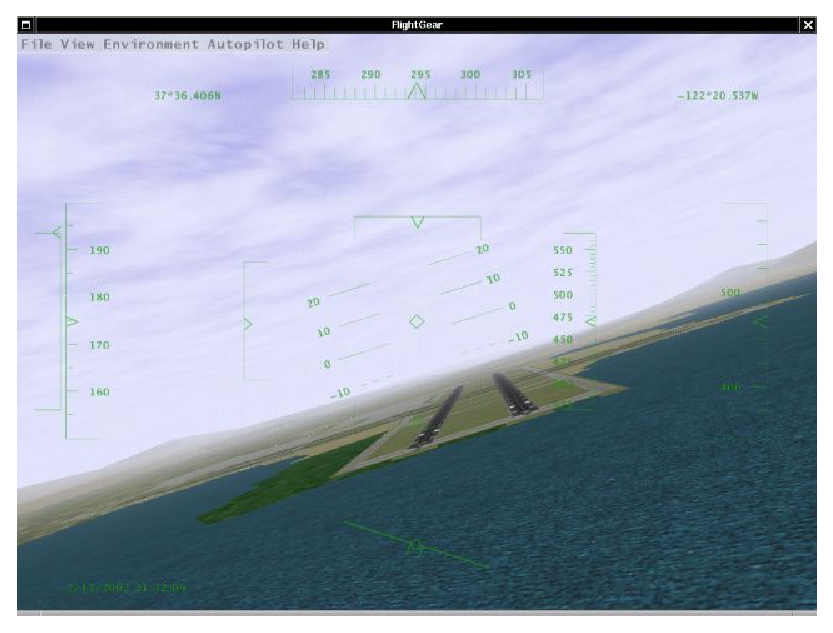
\includegraphics[clip,width=12.5cm]{KSFOapp}
}}

\smallskip
 \noindent
\ifchinese
图 1:UNIX 系统下的 \FlightGear{}:\textit{旧金山国际机场的糟糕进近——来自本手册一位作者的截图\ldots}
\fi
%\IfLanguageName{english}{
%Fig.\,1: \FlightGear{} under UNIX: \textit{Bad approach to San Francisco International - by one of the authors of this manual\ldots}
%}{}
\IfLanguageName{french}{
Image 1 : \FlightGear{} sous UNIX: \textit{mauvaise approche de l'a\'{e}roport de San Francisco International, par l'un des auteurs de ce manuel\ldots}
}{}
\IfLanguageName{italian}{
Fig. 1: FlightGear sotto UNIX: cattivo approccio al San Francisco International – scatto fatto da uno degli autori di questo manuale...
}{}

%%%%%%%%%%%%%%%%%%%%%%%%%%%%%%%%%%%%%%%%%%%%%%%%%%%%%%%%%%%%%%%%%%%%%%%%%%%%%%%%%%%%%%%%%%%%%%%
\ifchines
\section{系统需求}\index{系统需求}
\fi
%\IfLanguageName{english}{
%\section{System Requirements}\index{system requirements}
%}{}
\IfLanguageName{french}{
\section{Pr\'{e}-requis syst\`{e}me}\index{system requirements}
}{}
\IfLanguageName{italian}{
\section{Requisiti di sistema}\index{system requirements}
}{}
%%%%%%%%%%%%%%%%%%%%%%%%%%%%%%%%%%%%%%%%%%%%%%%%%%%%%%%%%%%%%%%%%%%%%%%%%%%%%%%%%%%%%%%%%%%%%%%

\ifchinese
与其他飞行模拟器相比,\FlightGear{} 的\Index{系统需求}并不奢侈。一个中等速度的 AMD Athlon64 或 Intel
P4 就可以,甚至是低端的 AMD Athlon/K7 或 Intel PIII 也都可以让 \FlightGear{} 做的非常好。你需要有一款适合的 3D 显卡。

运行 \FlightGear{} 有一个很重要的条件,就是需要一款支持 \Index{OpenGL} 的显卡。如果你不知道什么是 \Index{OpenGL} 可以参考 OpenGL 网站的简介
\fi
%\IfLanguageName{english}{
%In comparison to other recent flight simulators, the \Index{system requirements} for
%\FlightGear{} are not extravagant. A medium speed AMD Athlon64 or Intel
%P4, even a decent AMD Athlon/K7 or an Intel PIII should be sufficient
%to handle \FlightGear{} pretty well, given you have a proper 3D \Index{graphics
%card}.
%
%One important prerequisite for running \FlightGear{} is a graphics card whose driver supports
%\Index{OpenGL}. If you don't know what \Index{OpenGL} is, the overview given at the OpenGL website
%}{}
\IfLanguageName{french}{
En comparaison avec d'autres simulateurs de vol r\'{e}cents, les \Index{pr\'{e}-requis syst\`{e}me}
de \FlightGear{} ne sont pas exag\'{e}r\'{e}s. Un processeur AMD Athlon64 de vitesse moyenne, ou un
Intel P4, ou m\^{e}me un AMD Athlon/K7 d\'{e}cent ou un Intel PIII devraient \^{e}tre suffisants pour
faire fonctionner \FlightGear{} assez bien, pour peu que vous ayez une \Index{carte graphique} 3D appropri\'{e}e.

Un des pr\'{e}-requis les plus importants pour faire fonctionner \FlightGear{} est une carte graphique dont le
pilote prenne en charge \Index{OpenGL}. Si vous ne savez pas ce qu'est \Index{OpenGL}, la vue d'ensemble propos\'{e}e
sur le site Internet d'OpenGL :
}{}
\IfLanguageName{italian}{
Rispetto ad altri recenti simulatori di volo, i requisiti di sistema per FlightGear non sono stravaganti. Un AMD
Athlon64 o Intel P4 di velocit\`{a} media, o comunque un discreto AMD Athlon/K7 o un Intel PIII dovrebbe essere
sufficiente per gestire FlightGear abbastanza bene, mentre invece la cosa pi\`{u} importante \`{e} avere una
scheda grafica supportata.
Un presupposto importante per l'esecuzione di FlightGear \`{e} una scheda grafica il cui driver supporti OpenGL.
Per chi non sapesse cosa \`{e} OpenGL, la panoramica fornita sul sito web
}{}
\medskip

\web{http://www.opengl.org}
\medskip

\noindent
\ifchinese
简单说:“OpenGL起步于1992年,现在已经成为支持 2D 和 3D 的工业级应用程序接口...”

\FlightGear{} 不会(且永远不会)运行于只支持 \Index{Direct3D}/\Index{DirectX} 的显卡。相比于 OpenGL,Direct3D 是私有接口,并限制在 Windows 操作系统。

你可能在一个 3D 显卡不支持 \Index{OpenGL} 硬件加速的电脑上运行 \FlightGear{} ——甚至系统都没有 3D 显卡。然而没有硬件加速的电脑,即便是最快速的也会崩溃。没有硬件加速时的典型情况是\Index{帧速率}会低于每秒1帧。

任何现代的 3D 显卡都会支持 \Index{OpenGL}。如果 \Index{Windows} 显卡驱动不能支持 OpenGL,请访问你的显卡厂家的网站。你需要注意的是有时候 OpenGL 的驱动\index{OpenGL!驱动}是由主板的厂商提供的,而不是显卡厂商。如果你想购买一款运行 \FlightGear{} 的显卡,推荐 NVIDIA GeForce 显卡,因为比 AMD/ATI 显卡对 OpenGL 有更好的支持。256MB 的独立显存就已经绰绰有余了——即便较少的显存也能让很多人玩 \FlightGear{} 很开心呢。

要安装和执行基本的地景,你需要大概 500MB \Index{硬盘空间}。如果你想自己编译程序,你还需要另外的 500MB 来放源代码和编译过程产生的临时文件。这还不包括开发环境,这取决于操作系统以及环境使用。Windows 用户大概需要 300MB 的额外空间来做开发环境。Linux 和其他 UNIX 机器所需的开发环境大多都已经安装好了,因此这些平台仅需很少的额外空间。

关于\Index{声音效果},任何适合的\Index{声卡}都足够了。因为设计灵活,在 \Index{Linux} 和 \Index{Windows} 平台下,\FlightGear{} 可以支持大部分的\Index{飞行摇杆}和\Index{驾驶盘},以及\Index{脚踏舵板}。\FlightGear{} 甚至还可以支持全动式的飞行座椅。

\FlightGear{} 主要是在 \Index{Linux} 下开发的,Linux是一个自由的 UNIX 克隆(包括了大量的 GNU 组件),与\FlightGear{} 有着一样的精神,也是由一群互联网上广泛的合作开发而成。\FlightGear{} 也可以在 \Index{Windows} 下运行,一部分开发也是在 Windows 平台下开发。在 Mac OS X 上构建 \FlightGear{} 也是可行的,与 UNIX/X11 工作站有一些区别。如果你已经安装了合适的\Index{编译器},\FlightGear{} 都可以在以上这些平台完成构建。主要的全平台支持的编译器是自由的 \Index{GNU C++} 编译器(Win32 系统下则是 \Index{Cygnus} \Index{Cygwin} 编译器)。

如果你想在 Mac OS X 系统下运行 \FlightGear{},你需要至少 Mac OS X 10.4。最低硬件需求是 Power PC G4 1.0GHz 或一台 Intel Mac。然而若想飞行的更舒服我们推荐 MacBook Pro,Intel iMac,Mac Pro 或 Power Mac (Power PC G5)。 
\fi
%\IfLanguageName{english}{
%says it best: ``Since its introduction in 1992, OpenGL has become the
%industry's most widely used and supported 2-D and 3D graphics application programming
%interface (API)...''.
%
%\FlightGear{} does not run (and will never run) on a graphics board which only supports
%\Index{Direct3D}/\Index{DirectX}. Contrary to OpenGL, Direct3D is a proprietary interface, being r%estricted to
%the Windows operating system.
%
%You may be able to run \FlightGear{} on a computer that features a 3D video card not
%supporting hardware accelerated \Index{OpenGL} -- and even on systems without 3D
%graphics hardware at all. However, the absence of hardware accelerated OpenGL support can bring
%even the fastest machine to its knees. The typical signal for missing hardware acceleration
%are \Index{frame rate}s below 1 frame per second.
%
%Any modern 3D graphics featuring \Index{OpenGL} support will do. For
%\Index{Windows} video card drivers that support OpenGL, visit the home page of your video
%card manufacturer. You should note that sometimes OpenGL drivers\index{OpenGL!drivers}
%are provided by the manufacturers of the graphics chip instead of by the makers of the
%board. If you are going to buy a graphics card for running \FlightGear{}, an NVIDIA GeForce
%card is recommended, as these tend to have better OpenGL support than AMD/ATI Radeon. 256MB
%of dedicated graphics memory will be more than adequate - many people run \FlightGear{} happily
%on less.
%
%To install the executable and basic scenery, you will need around 500 MB of free \Index{disk
%space}. In case you want/have to compile the program yourself you will need about another
%500 MB for the source code and for temporary files created during compilation. This does not
%include the development environment, which will vary in size depending on the operating system
%and environment being used.  Windows users can expect to need approximately 300 MB of additional
%disk space for the development environment.  Linux and other UNIX machines should have most of
%the development tools already installed, so there is likely to be little additional space
%needed on those platforms.
%
%For the \Index{sound effects}, any capable \Index{sound card} should suffice.
%Due to its flexible design, \FlightGear{} supports a wide range of \Index{joysticks} and
%\Index{yokes} as well as \Index{rudder pedals} under \Index{Linux} and \Index{Windows}.
%\FlightGear{} can also provide interfaces to full-motion flight chairs.
%
%\FlightGear{} is being developed primarily under \Index{Linux}, a free UNIX clone
%(together with lots of GNU utilities) developed cooperatively over the Internet in much
%the same spirit as \FlightGear{} itself. \FlightGear{} also runs and is partly developed
%under several flavors of \Index{Windows}. Building \FlightGear{} is also possible on a Mac OS X
%and several different UNIX/X11 workstations. Given you have a proper \Index{compiler} installed,
%\FlightGear{} can be built under all of these platforms. The primary compiler for all platforms is
%the free \Index{GNU C++} compiler (the \Index{Cygnus} \Index{Cygwin} compiler under Win32).
%
%If you want to run \FlightGear under Mac OS X, you need to have Mac OS X 10.4 or higher.
%Minimum hardware requirement is either a Power PC G4 1.0GHz or an Intel Mac, but We suggest
%you have MacBook Pro, Intel iMac, Mac Pro, or Power Mac (Power PC G5) for comfortable flight.
%}{}

\IfLanguageName{french}{
l'explique tr\`{e}s bien : ``Depuis son introduction en 1992, OpenGL est devenue l'interface de
programmation d'application (Application Programming Interface, API) 2D et 3D la plus employ\'{e}e et
la mieux prise en charge de l'industrie...''.

\FlightGear{} ne fonctionne pas (et ne fonctionnera jamais) sur une carte graphique ne prenant en charge que \Index{Direct3D}/\Index{DirectX}.
Contrairement \`{a} OpenGL, Direct3D est une interface propri\'{e}taire, \'{e}tant limit\'{e}e au syst\`{e}me d'exploitation
Windows.

Vous devriez pouvoir faire fonctionner \FlightGear{} sur un ordinateur dot\'{e} d'une carte graphique 3D ne
prenant pas en charge l'acc\'{e}l\'{e}ration mat\'{e}rielle \Index{OpenGL} (et m\^{e}me sur des syst\`{e}mes sans
mat\'{e}riel graphique 3D du tout). Cependant, l'absence de prise en charge mat\'{e}rielle de l'acc\'{e}l\'{e}ration
OpenGL peut mettre sur les genoux m\^{e}me la plus rapide des machines. Les sympt\^{o}mes typiques de l'absence
d'acc\'{e}l\'{e}ration mat\'{e}rielle sont des \Index{taux d'images} (frame rate) inf\'{e}rieurs \`{a} 1 image par seconde.

Toute carte graphique 3D moderne prenant en charge \Index{OpenGL} fera l'affaire. Pour les pilotes de
carte graphique \Index{Windows} qui prennent en charge OpenGL, visitez la page d'accueil de votre fabricant de
carte vid\'{e}o. Notez que, parfois, les pilotes OpenGL\index{OpenGL!drivers} sont fournis par les fabricants
des processeurs graphiques et non par les fabricants des cartes. Si \^{e}tes sur le point d'acheter une carte
graphique pour faire fonctionner \FlightGear{}, une carte NVIDIA GeForce est recommand\'{e}e, car elles ont
tendance \`{a} b\'{e}n\'{e}ficier d'une meilleure prise en charge OpenGL que les cartes AMD/ATI Radeon. 256 Mo
de m\'{e}moire graphique d\'{e}di\'{e}e sera plus qu'appropri\'{e} - de nombreuses personnes font fonctionner
\FlightGear{} sans souci avec moins.

Pour installer les ex\'{e}cutables et les sc\`{e}nes par d\'{e}faut, vous aurez besoin d'environ 500 Mo
d'\Index{espace disque} libre. Au cas o\`{u} vous voudriez/deviez compiler le programme vous-m\^{e}me, vous
aurez besoin d'\`{a} peu pr\`{e}s 500 Mo suppl\'{e}mentaires pour le code source et pour les fichiers temporaires
cr\'{e}\'{e}s durant la compilation. Cel\`{a} ne comprend pas l'environnement de d\'{e}veloppement, qui variera
en taille en fonction du syst\`{e}me d'exploitation et de l'environnement utilis\'{e}s. Les utilisateurs de Windows
peuvent s'attendre \`{a} avoir besoin d'approximativement 300 Mo d'espace disque suppl\'{e}mentaire pour l'environnement
de d\'{e}veloppement. Les machines fonctionnant sous Linux ou autres UNIX devraient avoir la plupart des outils de
d\'{e}veloppement d\'{e}j\`{a} install\'{e}s, il est donc probable qu'il ne faille que peu d'espace disque suppl\'{e}mentaire
sur ces plate-formes.

En ce qui concerne les \Index{effets sonores}, n'importe quelle \Index{carte graphique} devrait suffir. En raison de sa
conception flexible, \FlightGear{} prend en charge une large un large \'{e}ventail de \Index{joysticks}, de
\Index{manches} et de \Index{palonniers} sous \Index{Linux} et \Index{Windows}.
\FlightGear{} peut \'{e}galement fournir des interfaces aux si\`{e}ges de vol \textit{full-motion}.

\FlightGear{} est d\'{e}velopp\'{e} principalement sous \Index{Linux}, un clone libre et gratuit d'UNIX
(ainsi qu'un bon nombre d'outils GNU) d\'{e}velopp\'{e} coop\'{e}rativement via Internet dans plus ou moins
le m\^{e}me esprit que \FlightGear{} lui-m\^{e}me. \FlightGear{} fonctionne \'{e}galement et est en partie d\'{e}velopp\'{e}
sous plusieurs versions de \Index{Windows}. Il est \'{e}galement possible de compiler \FlightGear{} sur Mac OS X
ainsi que sur diverses stations de travail UNIX/X11. D\`{e}s l'instant o\`{u} vous disposez d'un \Index{compilateur} appropri\'{e}
install\'{e}, \FlightGear{} peut-\^{e}tre compil\'{e} sous toutes ces plate-formes. Le principal compilateur sur toutes ces plateformes
est le compilateur libre \Index{GNU C++} (le compilateur \Index{Cygnus} \Index{Cygwin} sous Win32).

Si vous voulez lancer \FlightGear{} sous Mac OSX, vous aurez besoin de Mac OS X 10.4 ou sup\'{e}rieur. Les pr\'{e}-requis minimums
sont soit un Power PC G4 \`{a} 1,0 GHz ou un Mac Intel, mais nous vous sugg\'{e}rons un MacBook Pro,
Intel iMac, Mac Pro ou Power Mac (Power PC G5) pour un confort de vol optimal.
}{}
\IfLanguageName{italian}{
afferma: ''Fin dalla sua introduzione nel 1992, \index{OpenGL} \`{e} diventata l'industria delle
pi\`{u} diffuse e supportate grafiche 2D/3D per le interfacce di programmazione delle
applicazioni (API)...''.

FlightGear non funziona su una scheda grafica che supporta solo Direct3D/DirectX.
Contrariamente a OpenGL, Direct3D \`{e} un'interfaccia proprietaria, essendo progettata
solo per il sistema operativo di Windows.

Si pu\`{o} comunque eseguire FlightGear su un computer che dispone di una scheda video
3D che non supporta l'accelerazione hardware OpenGL - e anche su sistemi senza un hardware
grafico 3D. Tuttavia, l'assenza di accelerazione hardware OpenGL pu\`{o} portare anche la
macchina pi\`{u} veloce in ginocchio. Il segnale tipico della mancante accelerazione hardware
\`{e} costituito da frame rate inferiori a 1 fotogramma al secondo.

Quasi tutte le moderne schede grafiche 3D sono dotate di supporto OpenGL. Per sapere se la
propria scheda grafica lo supporta, visitare la homepage del produttore della scheda video.
Si richiama l'attenzione sul fatto che a volte i driver OpenGL sono forniti dai produttori
di chip grafici anzich\'{e} che dai creatori della scheda madre. Se avete intenzione di
acquistare una scheda grafica per l'esecuzione di FlightGear, \`{e} consigliabile una scheda
NVIDIA GeForce, in quanto \`{e} pi\`{u} probabile che supporti OpenGL rispetto ad un AMD/ATI
Radeon.
256MB di memoria grafica dedicata sono pi\`{u} che adeguati - molte persone usano FlightGear
tranquillamente anche con meno.

Per installare il paesaggio eseguibile e di base, avrete bisogno di circa 500 MB di spazio
libero sul disco. Nel caso in cui si voglia/debba compilare il programma da soli saranno
necessari circa altri 500 MB per il codice sorgente e per i file temporanei creati durante
la compilazione. Questo non include l'ambiente di sviluppo, che varia in dimensioni a seconda
del sistema operativo e all'ambiente informatico in uso. Gli utenti Windows possono aspettarsi
di avere bisogno di circa 300 MB di spazio aggiuntivo sul disco per l'ambiente di sviluppo.
Linux e altri sistemi UNIX dovrebbero avere la maggior parte degli strumenti di sviluppo
gi\`{a} installati, quindi \`{e} probabile che sia richiesto meno spazio su queste piattaforme.

Per gli \index{effetti sonori}, qualsiasi \index{scheda audio} dovrebbe essere sufficiente.
Grazie al suo design flessibile, FlightGear supporta una vasta gamma di joystick e periferiche,
come ad esempio le pedaliere.

FlightGear \`{e} stato sviluppato principalmente sotto Linux, un clone di UNIX libero (insieme
con un sacco di GNU utility) sviluppata cooperativamente su Internet pi\`{u} o meno con lo stesso
spirito di FlightGear. FlightGear \`{e} in parte sviluppato anche sotto varie versioni di Windows,
Mac OS X e diverse postazioni di lavoro Unix/X11. Una volta installati i programmi di sviluppo,
FlightGear pu\`{o} essere sviluppato sotto tutte queste piattaforme.

Il compilatore primario per tutte le piattaforme \`{e} la libera GNU C++ compiler (compilatore
Cygnus Cygwin sotto Win32).

Se si desidera eseguire FlightGear sotto Mac OS X, \`{e} necessario disporre di Mac OS X 10.4 o
superiore. I requisiti minimi hardware richiedono un 1,0 GHz G4 Power PC o un Mac Intel, ma vi
consigliamo di avere MacBook Pro, iMac Intel, Mac Pro, o Power Mac (G5 Power PC) per un volo
confortevole.
}{}

%%%%%%%%%%%%%%%%%%%%%%%%%%%%%%%%%%%%%%%%%%%%%%%%%%%%%%%%%%%%%%%%%%%%%%%%%%%%%%%%%%%%%%%%%%%%%%%
\ifchinese
\section{选择版本}\index{FlightGear!版本}
\fi
%\IfLanguageName{english}{
%\section{Choosing A Version}\index{FlightGear!versions}
%}{}
\IfLanguageName{french}{
\section{Choisir une version}\index{FlightGear!versions}
}{}
\IfLanguageName{italian}{
\section{La scelta di una versione}\index{FlightGear!versions}
}{}
%%%%%%%%%%%%%%%%%%%%%%%%%%%%%%%%%%%%%%%%%%%%%%%%%%%%%%%%%%%%%%%%%%%%%%%%%%%%%%%%%%%%%%%%%%%%%%%
\ifchinese
建议你运行官方发布的最新版本,每年都会发布,且可以通过以下方式获取已经编译好的二进制文件
\fi
%\IfLanguageName{english}{
%It is recommended that you run the latest official release, which are typically produced annually,
%and which are used to create the the pre-compiled binaries. It is available from
%}{}

\IfLanguageName{french}{
Nous vous recommandons d'utiliser la derni\`{e}re version officielle, g\'{e}n\'{e}ralement produite
annuellement et qui est utilis\'{e}e pour cr\'{e}er les binaires pr\'{e}-compil\'{e}. Elle est disponible
\`{a} l'adresse :
}{}
\IfLanguageName{italian}{
Si consiglia di installare l'ultima versione ufficiale disponibile al sito :
}{}

\medskip

\web{http://www.flightgear.org/Downloads/}

\IfLanguageName{italian}{
, che \`{e} solitamente prodotta annualmente, e che viene utilizzata per creare i file binari pre-compilati.
}{}

\medskip
\ifchinese
如果你想获得最新的、最完整(当然同时也是 bug 最多的)的代码,你可以从以下地址克隆
\fi
%\IfLanguageName{english}{
%If you really want to get the very latest and greatest (and, at times,
%buggiest) code, you can clone the sources at
%}{}
\IfLanguageName{french}{
Si vous voulez vraiment obtenir la toute derni\`{e}re version du code (la plus \'{e}volu\'{e}e et, parfois, la plus
instable), vous pouvez cloner les sources \`{a} partir de l'adresse :
}{}
\IfLanguageName{italian}{
Se davvero si vuole ottenere l'ultima versione (generalmente \`{e} anche la pi\`{u} buggata), \`{e} possibile
clonare i sorgenti pi\`{u} recenti all'indirizzo
}{}
 \medskip

\web{http://www.gitorious.org/fg}. \footnote{译者注:因为 Gitorious 网站已经关闭,从2015年3月起代码已经转移到 \web{https://sourceforge.net/projects/flightgear/}}

\ifchinese
想获取这些的代码,可以看这个介绍如何获取 \FligtGear{} 的代码仓库
\fi
%\IfLanguageName{english}{
%to get the recent code. A detailed description of how to set this up for \FlightGear{}
%can be found at
%}{}
\IfLanguageName{french}{
pour obtenir le code le plus r\'{e}cent. Une description d\'{e}taill\'{e}e de la pr\'{e}paration de code en vue de l'ex\'{e}cution de
\FlightGear{} peut \^{e}tre trouv\'{e}e \`{a} l'adresse :
}{}
\IfLanguageName{italian}{
Istruzioni dettagliate su come farlo possono essere trovate qui:
}{}
 \medskip

\web{http://wiki.flightgear.org/GIT}.



%%%%%%%%%%%%%%%%%%%%%%%%%%%%%%%%%%%%%%%%%%%%%%%%%%%%%%%%%%%%%%%%%%%%%%%%%%%%%%%%%%%%%%%%%%%%%%%
\ifchinese
\section{飞行动态模型\label{flightmodels}}\index{flight dynamics model 飞行动态模型}\index{flight model 飞行模式}
\fi
%\IfLanguageName{english}{
%\section{Flight Dynamics Models\label{flightmodels}}\index{flight dynamics model}\index{flight model}
%}{}
\IfLanguageName{french}{
\section{Mod\`{e}les de dynamique de vol (Flight Dynamics Models, FDM)\label{flightmodels}}\index{Mod\`{e}les de dynamique de vol}\index{flight model}
}{}
\IfLanguageName{italian}{
\section{Modelli di volo dinamici\label{flightmodels}}\index{Mod\`{e}les de dynamique de vol}\index{flight model}
}{}
%%%%%%%%%%%%%%%%%%%%%%%%%%%%%%%%%%%%%%%%%%%%%%%%%%%%%%%%%%%%%%%%%%%%%%%%%%%%%%%%%%%%%%%%%%%%%%%
\ifchinese
历史上,
\fi
\IfLanguageName{english}{
Historically, \FlightGear{} was based on a flight model it inherited (together
with the Navion airplane) from LaRCsim. As this had several limitations (most importantly,
many characteristics were hard wired in contrast to using configuration files), there were
several attempts to develop or include alternative \Index{flightmodels}. As a result,
\FlightGear{} supports several different flight models, to be chosen from at runtime.
}{}
\IfLanguageName{french}{
Historiquement, \FlightGear{} \'{e}tait bas\'{e} sur un mod\`{e}le de vol qu'il a h\'{e}rit\'{e} de LaRCsim (ainsi que l'avion Navion). Comme cela imposait plusieurs limitations (la plus importante, beaucoup de caract\'{e}ristiques
\'{e}taient cod\'{e}es en dur au lieu de passer par des fichiers de configuration), quelques tentatives ont
\'{e}t\'{e} faites pour d\'{e}velopper ou inclure des mod\`{e}les de vol alternatifs. En cons\'{e}quence,
\FlightGear{} prend aujourd'hui en charge diff\'{e}rents mod\`{e}les de vol, qui doivent \^{e}tre choisis au lancement
de l'application.
}{}
\IfLanguageName{italian}{
Storicamente, FlightGear \`{e} basato su un modello di volo che ha ereditato (insieme con la
Navion Airplane) dalla LaRCsim. Dato che questi aveva molte limitazioni (soprattutto, molte
caratteristiche erano cablate in contrasto con i file di configurazione), ci sono stati diversi
tentativi di sviluppare o includere modelli di volo alternativi. Come risultato finale, FlightGear
supporta diversi modelli di volo differenti, da scegliere in fase di esecuzione.
}{}

\begin{itemize}
\IfLanguageName{english}{
\item Possibly the most important one is the JSB flight model developed by Jon Berndt. The JSB
flight model is part of a stand-alone project called \JSBSim:
}{}
\IfLanguageName{french}{
\item Le plus important est probablement le mod\`{e}le de vol JSB d\'{e}velopp\'{e} par Jon Berndt. Le mod\`{e}le
de vol JSB fait partie d'un projet autonome appel\'{e} \JSBSim:
}{}
\IfLanguageName{italian}{
\item Forse il pi\`{u} importante \`{e} il modello di volo JSB sviluppato da Jon Berndt. Il modello di volo
JSB \`{e} parte di un progetto autonomo denominato \JSBSim:
}{}

\web{http://jsbsim.sourceforge.net/}.

\IfLanguageName{english}{
\item Andrew Ross created another flight model called \YASim{}\index{YASim} for
\textit{Yet Another Simulator}. \YASim{} takes a fundamentally different approach to many other FDMs by
being based on geometry information rather than aerodynamic coefficients. \YASim{} has a particularly
advanced helicopter FDM.
}{}
\IfLanguageName{french}{
\item Andrew Ross a cr\'{e}\'{e} un autre mod\`{e}le de vol appel\'{e} \YASim{}\index{YASim} pour
\textit{Yet Another Simulator} (encore un autre simulateur). \YASim{} prend une approche fondamentalement diff\'{e}rente
de nombreux autres FDM, car il se base sur l'information g\'{e}om\'{e}trique plut\^{o}t que sur les coefficients a\'{e}rodynamiques.
\YASim{} dispose d'un FDM particuli\`{e}rement avanc\'{e} pour les h\'{e}licopt\`{e}res.
}{}
\IfLanguageName{italian}{
\item Andrew Ross ha creato un altro modello di volo chiamato \YASim{}. Quest'ultimo ha un approccio
fondamentalmente diverso da molti altri modelli di volo, essendo basato su informazioni geometriche
piuttosto che su coefficienti aerodinamici. \YASim{} ha anche un modello di volo per elicotteri
particolarmente avanzato.
}{}

\IfLanguageName{english}{
\item Christian Mayer developed a flight model of a hot air
balloon. Curt Olson subsequently integrated a special ``UFO'' slew mode, which
helps you to quickly fly from point A to point B.
}{}
\IfLanguageName{french}{
\item Christian Mayer a d\'{e}velopp\'{e} le mod\`{e}le de vol d'un ballon \`{a} air chaud. Curt Olson int\'{e}gra ensuite un mode
de d\'{e}placement sp\'{e}cial, appel\'{e} ``UFO'', qui vous aide \`{a} voler rapidement d'un point A \`{a} un point B.
}{}
\IfLanguageName{italian}{
\item Christian Mayer ha sviluppato un modello di volo di una mongolfiera. Curt Olson successivamente
ha integrato una speciale modalit\`{a} ``UFO'', che aiuta a volare rapidamente dal punto A al punto B.
}{}

\IfLanguageName{english}{
\item Finally, there is the \Index{UIUC flight model}, developed by a
team at the University of Illinois at Urbana-Champaign. This work was
initially geared toward modeling aircraft in icing conditions\index{icing!modelling}, but now
encompasses ``nonlinear'' aerodynamics, which result in more realism
in extreme attitudes, such as stall and high angle of attack flight.  Two
good examples that illustrate this capability are the \Index{Airwave Xtreme 150}
\Index{hang glider} and the 1903 \Index{Wright Flyer}. More details of the UIUC
flight model can be found at
}{}
\IfLanguageName{french}{
\item Enfin, il existe le \Index{mod\`{e}le de vol UIUC}, d\'{e}velopp\'{e} par une \'{e}quipe de
l'Universit\'{e} d'Illinois \`{a} Urbana-Champaign. Ce travail \'{e}tait initialement
tourn\'{e} vers la mod\'{e}lisation d'un a\'{e}ronef rencontrant des conditions de givrage\index{icing!modelling},
mais il inclut maintenant l'a\'{e}rodynamique ``non-lin\'{e}aire'', qui a pour cons\'{e}quence d'am\'{e}liorer le
r\'{e}alisme dans des attitudes extr\`{e}mes, comme le d\'{e}crochage et les vols \`{a} angle d'attaque \'{e}lev\'{e}.
Deux bons exemples qui illustrent cette capacit\'{e} sont le \Index{deltaplane} \Index{Airwave Xtreme 150} et le \Index{Wright Flyer} de 1903. De plus amples d\'{e}tails du mod\`{e}le de vol UIUC peuvent \^{e}tre obtenus \`{a} l'adresse :
}{}
\IfLanguageName{italian}{
Infine, vi \`{e} il \Index{modello di volo UIUC}, sviluppato da un team della University of Illinois a Urbana-Champaign.
Questo lavoro \`{e} stato inizialmente orientato verso i modellini di aeromobili, ma ora comprende anche
aerodinamiche ``non lineari'', che si traducono in un maggiore realismo negli atteggiamenti estremi, come nello
stallo e negli alti angoli di attacco in volo.
Due buoni esempi che illustrano questa capacit\`{a} sono il \index{deltaplano} \Index{Airwave Xtreme 150} e il 1903 \Index{Wright Flyer}.
Maggiori dettagli sul modello di volo UIUC sono disponibili all'indirizzo
}{}

\web{http://www.ae.illinois.edu/m-selig/apasim/Aircraft-uiuc.html}
\end{itemize}
\IfLanguageName{english}{
It is even possible to drive FlightGear's scene display using an external
FDM\index{FDM!external} running on a different computer or via named
pipe\index{FDM!pipe} on the local machine -- although this might not be a
setup recommended to people just getting in touch with \FlightGear{}.
}{}
\IfLanguageName{french}{
Il est m\^{e}me possible de piloter l'affichage de la sc\`{e}ne de \FlightGear{}
en utilisant un FDM externe\index{FDM!external} fonctionnant sur un ordinateur diff\'{e}rent ou
par l'interm\'{e}diaire d'un canal nomm\'{e} sur la machine locale (bien que cela ne soit pas
recommand\'{e} aux utilisateurs d\'{e}couvrant \FlightGear{}).
}{}
\IfLanguageName{italian}{
\'{E} anche possibile visualizzare le scene di FlightGear con un modello di volo esterno
in esecuzione su un computer diverso o tramite named pipe sulla macchina locale - anche se
questo potrebbe non essere una configurazione consigliata per le persone che vogliono solo
entrare in contatto con FlightGear.
}{}

%%%%%%%%%%%%%%%%%%%%%%%%%%%%%%%%%%%%%%%%%%%%%%%%%%%%%%%%%%%%%%%%%%%%%%%%%%%%%%%%%%%%%%%%%%%%%%%
\IfLanguageName{english}{
\section{About This Guide}
}{}
\IfLanguageName{french}{
\section{A propos de ce guide}
}{}
\IfLanguageName{italian}{
\section{Informazioni su questa guida}
}{}
%%%%%%%%%%%%%%%%%%%%%%%%%%%%%%%%%%%%%%%%%%%%%%%%%%%%%%%%%%%%%%%%%%%%%%%%%%%%%%%%%%%%%%%%%%%%%%%

\IfLanguageName{english}{
\markright{\thesection.\hspace*{1mm} ABOUT THIS GUIDE}

There is little, if any, material in this Guide that is presented here exclusively. You
could even say with Montaigne that we ``merely gathered here a big bunch of other men's
flowers, having furnished nothing of my own but the strip to hold them together''. Most
(but fortunately not all) of the information herein can also be obtained from the
\FlightGear{} web site\index{FlightGear Website} located at
}{}

\IfLanguageName{french}{
\markright{\thesection.\hspace*{1mm} A PROPOS DE CE GUIDE}

Il y a peu, voire pas, de ressources dans ce guide qui y soient exclusivement pr\'{e}sent\'{e}es.
Vous pourriez m\^{e}me dire comme Montaigne ``Je n'ai fait qu'un bouquet de fleurs et n'ai rien fourni
de moi-m\^{e}me que le lien qui les assemble.'' La majeure partie (mais heureusement pas
l'int\'{e}gralit\'{e}) des informations pr\'{e}sentes ici peut \'{e}galement \^{e}tre obtenue
\`{a} partir du site Internet de \FlightGear{} situ\'{e} \`{a} l'adresse :
}{}
\IfLanguageName{italian}{
In questa guida c'\`{e} poco materiale. Altre informazioni aggiuntive sono presenti sul sito web di
\FlightGear{}
}{}

\medskip

\web{http://www.flightgear.org/}
\medskip

\IfLanguageName{english}{
\textit{The \FlightGear{} Manual} is intended to be a first step
towards a complete \FlightGear{} documentation\index{FlightGear
documentation}. The target audience is the end-user who is not
interested in the internal workings of \Index{OpenGL} or in building
his or her own scenery. It is our hope that someday there will be an
accompanying \textit{\FlightGear{} Programmer's Guide}\index{FlightGear
Programmer's Guide}
a \textit{\FlightGear{} Scenery Design Guide},\index{FlightGear Scenery Design Guide}
describing the Scenery tools now packaged as \TerraGear{}; and a \textit{\FlightGear{}
Flight School}\index{FlightGear Flight School} package.
 \medskip

\textbf{We kindly ask you to help us refine this document by submitting corrections,
improvements, suggestions and translations. All users are invited to contribute
descriptions of alternative setups (graphics cards, operating systems
etc.). We will be more than happy to include those in future versions
of \textit{The FlightGear Manual} (of course not without giving credit
to the authors).}
}{}

\IfLanguageName{french}{
\textit{Le manuel \FlightGear{}} a pour vocation d'\^{e}tre un premier pas vers une
documentation compl\`{e}te de \FlightGear{}\index{FlightGear documentation}. Il s'adresse
\`{a} l'utilisateur final qui n'est pas int\'{e}ress\'{e} par le fonctionnement interne
d'\Index{OpenGL} ou par la cr\'{e}ation de ses propres sc\`{e}nes. Nous esp\'{e}rons qu'un
jour il y aura, pour accompagner ce document, un \textit{Guide du programmeur de \FlightGear{}}\index{FlightGear
Programmer's Guide}, un \textit{Guide de cr\'{e}ation des sc\`{e}nes de \FlightGear{}},\index{FlightGear Scenery Design Guide}
d\'{e}crivant les outils de sc\`{e}nes actuellement livr\'{e}s avec \TerraGear{}; et un paquetage \textit{Ecole de pilotage \FlightGear{}}\index{Ecole de pilotage FlightGear}.
 \medskip

\textbf{Merci de nous aider \`{a} am\'{e}liorer ce document en nous soumettant vos corrections, am\'{e}liorations, suggestions et traductions.
Tous les utilisateurs sont invit\'{e}s \`{a} contribuer aux descriptions des configurations alternatives (cartes graphiques, syst\`{e}mes d'exploitation, etc.). Nous serons plus qu'heureux de les inclure dans les futures versions du \textit{manuel FlightGear} (bien entendu sans oublier le cr\'{e}dit attribuable \`{a} leurs auteurs).}
}{}
\IfLanguageName{italian}{
Il Manuale FlightGear \`{e} destinato ad essere un primo passo verso una completa documentazione di FlightGear.

Non abbiamo riportato tutte le informazioni qui, perch\'{e} questo documento \`{e} destinato all'utente finale,
che si presume non sia interessato al funzionamento interno di OpenGL n\'{e} tanto meno alla programmazione del
simulatore. \`{e} nostra speranza che un giorno, assieme al pacchetto base di FlightGear, sia integrato anche un
manuale per i programmatori, gli sviluppatori e i disegnatori di scenari.

Vi preghiamo di aiutarci a perfezionare questa guida inviandoci correzioni, miglioramenti, suggerimenti e traduzioni.
Tutti gli utenti sono invitati a contribuire anche nelle descrizioni di configurazioni alternative (schede grafiche,
sistemi operativi, ecc). Saremo pi\`{u} che felici di includere questi nelle future versioni del
Manuale di FlightGear (ovviamente non senza dare credito agli autori).
}{}

%% Revision 0.00  1998/09/08  michael
%% Initial revision for version 0.53.
%% Revision 0.01  1998/09/20  michael
%% several extensions and corrections
%% revision 0.10  1998/10/01  michael
%% final proofreading for release
%% revision 0.11  1998/11/01  michael
%% minor corrections on platforms, satellite data, OpenGL
%% added Navion pic
%% revision 0.12  1999/03/07  michael
%% update on recent development
%% revision 0.20  1999/06/04  michael
%% updates on recent development, corrections of links
%% revision 0.3 2000/04/20 michael
%% Rewritten for version 0.7.2, many changes, added development since summer 1999,
%% development vs. stable version, split into SimGear/FlightGear/TerraGear
%% Proofread by Jon Berndt
%% revision 0.4 2001/05/12 michael
%% update on development during the last year, corrections on requirements,
%% new sections on different versions and on flight models
%% revision 0.41 2001/07/01 martin & michael
%% comment on external FDM
%% hint to FAQ
%% extended remarks on property manager
%% revision 0.5 2002/01/01 michael
%% several minor updates, corrected links
%% Hint on YASim by Martin
%% Picture KSFOapp added by Martin
%% System requirements contributed from Darrell
%% revision 0.6 2002/02/23 cameron
%% Many, many corrections
%% Rewrote several parts
%% Changed section titles
%% revision 0.6 2002/09/07 michael
%% Added contribution by M Selig on UIUC models
%% 3 minor typo/grammar edits by Dave Perry
%% (P.12 replaced double apostrophe, p.14 <<<to to  >>> to, <<<users is >>>users are
%% Revision 16/10/08: spelling, grammar, syntax and typo corrections.
